\section{File System}

Para el sistema de archivos elegí implementar a MinixFs o mfs (similar a ext2).

La parte más interesante de un sistema de archivos tipo Unix como lo es mfs es
la idea de inodos. Básicamente todo archivo (y como archivo contemplamos también
a directorios/pipes/links/etc.) es representado por un inodo. Un inodo esta
compuesto por una serie de campos que definen el archivo, y luego referencias a
los bloques en donde se encuentran sus datos, en el caso de tenerlos.

La función principal de un inodo es referenciar todos los bloques que conforman
un archivo. Lo bueno de este método es que al abrir y leer un archivo, solo es
necesario mirar a su inodo, éste tiene toda la información necesaria para
leerlo. Esto es una mejora substancial comparado con sistemas del tipo FAT, que
requieren de una tabla aparte con la información de todos los archivos. En este
último caso una tabla de este estilo sería enorme para los tamaños de los discos
en la actualidad, y ocuparía varios Mbyes en memoria constantemente. En cambio
con inodos solo es necesario mantener en memoria aquellos que se encuentran
actualmente en uso, aprovechando mejor los recursos.

A continuación se muestra un gráfico con la estructura general de un inodo en
mfs (similar a los inodos en ext2 o cualquier otro fs tipo unix):

\begin{center}
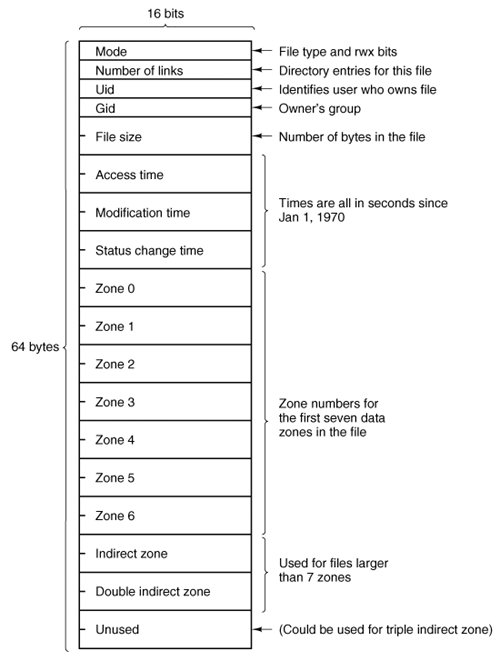
\includegraphics[scale=0.6]{../img/inode.png}
\end{center}

Esta imagen (al igual que el resto de las utilizadas en esta sección MinixFS)
fue tomada del libro de Tanembaum, y contiene descripciones de los
campos que conforman el inodo: 'mode' que nos da el tipo de archivo y sus
atributos de lectura/escritura/ejecución; 'links' nos dice cuantos directorios
contienen al archivo (es decir cuantos 'hard links' existen); 'uid/gid' el dueño
y su grupo; 'size' el tamaño; 'access/mod/status time' tiempos varios; 'zone
0-6' los punteros a los primeros 7 bloques del archivo.

Paramos aquí para comentar una característica de los inodos. Para poder contar
con archivos suficientemente grandes, se implemento la idea de bloques
indirectos/doble indirectos/triple indirectos. En caso de que la
información del archivo supere el espacio que proveen los primeros 7 bloques
referenciados en el inodo, se pasa al bloque de indirectos, que consta de un
bloque completo con punteros a otros bloques donde sigue el archivo. En caso de
que éste último no alcanze, se repite la idea y se utiliza el doble indirecto,
que apunta a un bloque con punteros a otros bloques, que a su vez contienen
punteros a bloques con la información. Para entender mejor el funcionamiento ver
el siguiente gráfico:

\begin{center}

\includegraphics[scale=0.62]{../img/inode_links.png}
\end{center}

De esta manera se logra expandir el límite del tamaño de un archivo los
suficiente como para que no sea un problema. En el caso de mfs los bloques
triple indirectos no son utilizados, pero el espacio en el inodo existe por si
fueran a ser necesarios en el futuro.

Veamos ahora como se implementan en nuestro sistema. El código de manejo de
inodos se encuentra en los archivos fs/inode.c y fs/inode.h, con partes menores
en fs/fs.c.

La función más interesante en el manejo de inodos es find\_inode(), que dado un
directorio de inicio y un path tipo unix (ej. jp/orga2/informe.pdf), encuentra y
devuelve el inodo buscado en caso de existir (en nuestro ejemplo sería el inodo
correspondiente al archivo informe.pdf). La implementación permite que se pueda
borrar el archivo en cuestion, se cree, o simplemente que se devuelva. Por
ejemplo, para conseguir el inodo correspondiente al archivo '/home/jp/hola.txt',
bastaría con llamar a la la función find\_inode(NULL, "/home/jp/hola.txt",
FS\_SEARCH\_GET).

Luego de decidir por donde empezar la busqueda (si el path empieza con '/'
empezamos en el root directory), esta función se encarga de ir componente por
componente navegando los directorios del path y avanzando hasta el último
subdirectorio. Logra esto utilizando la función search\_inode(), que dado un
directorio y un nombre de archivo, devuelve el numero inodo correspondiente, en
caso de que exista.

Analicemos más de cerca esta última función. Comienza recorriendo un
directorio entrada por entrada buscando aquella que coincide con el nombre de
archivo/carpeta buscado. Hace uso de varias funciones auxiliares que
detallaremos a continuación. El siguiente extracto de código de search\_inode()
muestra el loop principal (simplificado):

\begin{verbatim}
    pos = 0;
    entries = dir->i_size / DIRENTRY_SIZE;
    for (i = 0; i < entries; ++i) {
        if ( (dentry = next_entry(dir, &pos)) == NULL)
            break;

        if (dentry->num != 0)
            if (mystrncmp(name, dentry->name, MAX_NAME) == 0)
                return dentry;
    }
\end{verbatim}

La manera en que el código recorre las entradas del directorio es mediante la
función read\_map(), que dado una posición de un archivo/carpeta, devuelve el
bloque en que se encuentra (es decir, resuelve bloques
directos/indirectos/etc.); esta es utilizada por next\_entry() para recorrer
los bloques del directorio. Así vamos bloque por bloque recorriendo
todas las entradas, comparando una por una con la función
mystrncmp (una imitación de strncmp de la biblioteca estandar, recordar que no
contamos con ninguna de estas funciones). En el caso de que no se encuentre la
entrada que se buscaba, search\_inode() devuelve NULL. En el caso de que
necesite una entrada vacía, se provee la función empty\_entry().

Es importante aclarar que hay una diferencia clave con la manera en que está
implementado mfs en minix. Funciones como get\_block(), que dado un número de
bloque, devuelve el puntero al mismo,  requieren llamar al
disco, recobrar el bloque en cuestión y guardarlo en memoria para poder
utilizarlo. En cambio nosotros simplemente apuntamos a la posición de dicho
bloque, ya que todo se encuentra pre-cargado. Lo mismo sucede con los inodos y
la función get\_inode(), en la implementación real del fs se mantiene una cache
de inodos que contiene todos aquellos que se están utilizando en ese momento,
lo cual no es necesario en nuestro caso por el mismo motivo.

\subsection{System Calls del FS}

Los sistemas tipo unix utilizan la idea de descriptor de archivo o 'fd' para
identificar archivos abiertos. Cuando un programa quiere abrir un archivo, se le
es entregado este fd, que no es más que un número identificador. Luego basta
utilizar este número para realizar cualquier acción sobre el archivo
(leer/escribir/etc.).

Las funciones de manipulación de fds se encuentran en los archivos fs/file.c y
fs/file.h. Cada proceso en su tabla contiene un arreglo con los fds y
sus respectivos inodos. Mediante las funciones get\_fd() y release\_fd(), uno
reserva y devuelve fds según las necesidades del proceso.

La implementación de estas funciones hace uso del archivo sys/queue.h, una
implementación estándar de listas para los sistemas unix. Declarando un par de
punteros en el arreglo de fds, simulamos una lista tipo fifo con la que nos
aseguramos que pedir y devolver fds sea siempre $O(1)$. En el caso de get\_fd()
tenemos:

\begin{verbatim}
int get_fd(struct inode_s *ino, unsigned int pos)
{
    struct unused_fd_t *unused_fd;
    struct file_s *file;

    if (current_process != NULL) {
        unused_fd = &current_process->unused_fd;
        file = LIST_FIRST(unused_fd);
        if (file != NULL)
            LIST_REMOVE(file, unused);
    } else {
        file = &tmpfile;
    }

    if (file != NULL) {
        file->f_ino = ino;
        file->f_pos = pos;
        return file->f_fd;
    }

    return ERROR;
}
\end{verbatim}

De esta manera podemos utilizar la idea de listas sin tener que agregar
complicaciones al código, y más que nada no tenemos que introducir memoria
dinámica, ya que los arreglos que simulan la lista son estáticos y por ende
fijos.

Con el manejo de fds completo, comienza el código que rearma todo lo ya
explicado para implementar las llamadas al sistema. Para cada system call unix,
la función que la recibe tiene el prefijo "fs\_" (por ejemplo, la función
fs\_open() atiende la llamada open()). Se implementaron las llamadas open(),
close(), write(), read(), lseek(), unlink() y rename() para manejo de archivos,
chdir(), mkdir(), rmdir() y getdents() para manejo de carpetas.

Las implementación de estas funciones se encuentra en los archivos fs/fs.c y
fs/fs.h. Veamos como se hicieron algunas de estas funciones.

Hay que tener en cuenta que para abstraer las llamadas a los archivos (si estos son dispositivos o
archivos comunes), la llamada open le asigna a la estructura del fd correspondiente su
file\_operations, luego las syscalls hacia lseek, write, read, etc. en realidad son wrappers que
llaman a la operación definida en esta escructura. Por ejemplo, en caso de abrir el archivo
/dev/tty0, las operaciones apuntarán a las funciones del driver tty.

Volviendo al fs, en el caso de read() y write(), comenzaron siendo funciones distintas, pero
rápidamente me di cuenta que el código entre ellas era muy similar, por lo que
decidí separarlo en la función fs\_readwrite(). Esta se encarga de leer o
escribir un archivo, dependiendo de la flag que se le provee. Hace algunos
checkeos importantes (como por ejemplo fijarse si el archivo no es un
dispositivo de caracteres), y luego llama a copy\_file() que realiza el
trabajo duro:

\begin{verbatim}
while (n > 0) {
    if ( (blocknr = read_map(ino, pos)) == NO_BLOCK)
        return ERROR;
    block = (char *) get_block(blocknr);

    off = pos % BLOCK_SIZE;
    size = MIN(n, BLOCK_SIZE - off);

    if (flag == FS_WRITE) mymemcpy(block + off, buf, size);
    else                  mymemcpy(buf, block + off, size);

    n -= size;
    pos += size;
    buf += size;
    release_block(block);
}
\end{verbatim}

El loop principal de copy\_file() va navegando los bloques del archivo con
read\_map() y, dependiendo si se busca leer o escribir, utiliza la función
mymemcpy para realizar el trabajo (que es un clon de la función de mismo nombre
de la biblioteca estándar).


En un principio las funciones search\_inode() y find\_inode() eran muy simples,
uno le daba un path y devolvian el inodo correspondiente. Cuando comenzé a
implementar las llamadas de sistema de directorios me di cuenta que
este método no iba a funcionar, y tenía dos opciones: o bien crear nuevas
funciones de manejo de inodos para directorios, o cambiar estas 2 y reordenar el
código. El problema de la primer opción es que mucho código se duplica, lo que
ensucia la implementación y por lo tanto no lo consideré. Luego tomé el segundo
camino, cambie la signatura de las funciones para que search\_inode() devuelva
la entrada misma en el directorio.

Utilizando esta modificación, rmdir() remueve un directorio asegurandose
primero que este vacío. Esto requiere de conseguir el inodo del padre y del
hijo, checker que este vacío y limpiar la entrada en el padre.

La llamada mkdir() no solo requiere crear el nuevo inodo de directorio, sino que
también hay que colocar los links a '.' y '..'; también rename() hace uso de
este cambio, toma las entradas del directorio viejo y del nuevo, y copia los
contenidos de una a la otra, además debe fijarse si se trata de un directorio,
para actualizar la referencia '..'; chdir() que cambia el directorio actual
(el inodo del directorio actual se guarda en la tabla del proceso).

Por último esta getdents(), que se utiliza para recorrer un directorio. Esta
llamada es media extraña (por esta razón se utiliza una mucho más amistosa en
POSIX, readdir(), que a su vez llama a getdents()), dado un buffer y un tamaño,
copia en este buffer la mayor cantidad de estructuras de entrada de directorio
posibles. El problema es que estas estructuras no tienen un tamaño fijo,
contienen el nombre del archivo que es variable. Por si esto no fuera poco,
esta estructura evolucionó con el tiempo en linux, y se le agregó al final de
todo, despues del nombre, un campo d\_type que dice si la entrada es un archivo
regular/directorio/dispositivo etc. Para recobrar esta información es necesario
calcular el tamaño de la estructura, sumarlo al inicio de la misma y castear el
valor de d\_type. Luego recorrer el buffer para el usuario puede ser un poco
trabajoso (ver la implementación del programa ls).

DISCLAMER: Esta sección la basé en otra entrega de este TP (Orga 2)
